\section{Metrics}

\begin{frame}{Reporting Posterior Metrics}

  \begin{itemize}
    \item By the end of 10 years, we report key metrics from the final posterior distribution.
    \item 95\% Confidence Interval: The range where the team’s win probability is most likely to lie.
    \item Posterior Mean: The expected win probability based on all 10 years of data.
    \item Standard Deviation: Reflects our confidence in this probability estimate; lower Standard Deviation implies greater certainty.
  \end{itemize}
  
\end{frame}

\begin{frame}{95\% Confidence Interval}

\begin{figure}
  \centering
  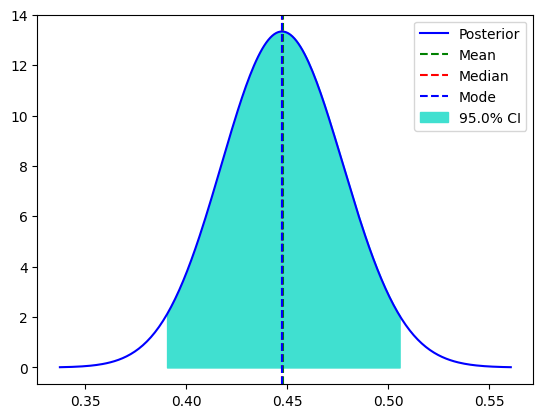
\includegraphics[width=.8\linewidth]{../Report/images/confidence-interval.png}
  \caption{95\% Confidence Interval}
\end{figure}
  
\end{frame}

\begin{frame}{Posterior Mean and Standard Deviation Analysis}

  \begin{itemize}
    \item The posterior mean over time shows how our estimate of win probability has evolved.
    \item A decreasing Standard Deviation suggests that our confidence is increasing, as we have more data to base our estimates on.
    \item These metrics help us assess how consistent the team’s performance has been over time.
  \end{itemize}
  
\end{frame}

\begin{frame}{Posterior Mean}
    
\begin{figure}
  \centering
  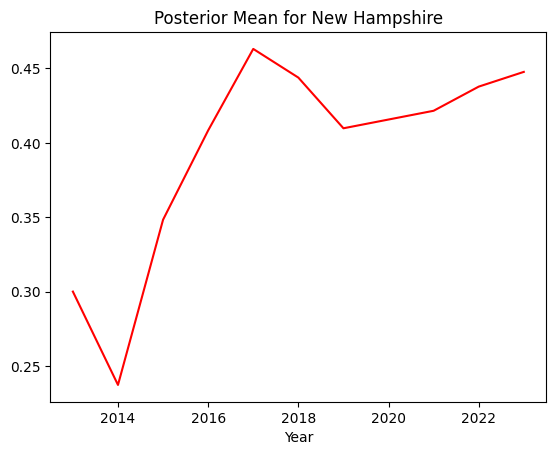
\includegraphics[width=.8\linewidth]{../Report/images/posterior-mean.png}
  \caption{Posterior Mean for each year}
\end{figure}

\end{frame}

\begin{frame}{Posterior Standard Deviation}

\begin{figure}
  \centering
  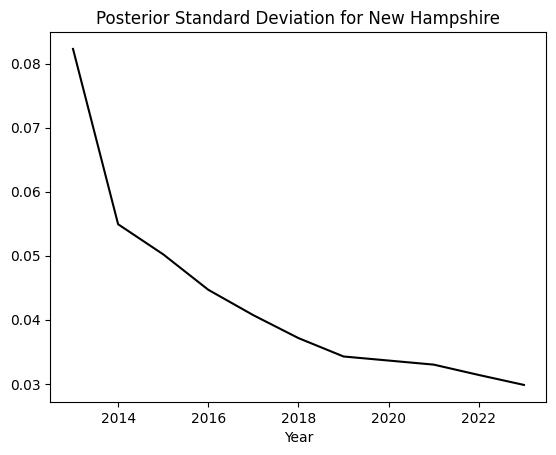
\includegraphics[width=.8\linewidth]{../Report/images/posterior-sd.png}
  \caption{Posterior Standard Deviation for each year}
\end{figure}

\end{frame}